\documentclass{report}
\usepackage{luatexja} % LuaTeXで日本語を使うためのパッケージ
\usepackage{luatexja-fontspec} % LuaTeX用の日本語フォント設定

% --- 数学関連 ---
\usepackage{amsmath, amssymb, amsfonts, mathtools, bm, amsthm} % 基本的な数学パッケージ
\usepackage{type1cm, upgreek} % 数式フォントとギリシャ文字
\usepackage{physics, mhchem} % 物理や化学の記号や式の表記を簡単にする

% --- 表関連 ---
\usepackage{multirow, longtable, tabularx, array, colortbl, dcolumn, diagbox} % 表のレイアウトを柔軟にする
\usepackage{tablefootnote, truthtable} % 表中に注釈を追加、真理値表
\usepackage{tabularray} % 高度な表組みレイアウト

% --- グラフィック関連 ---
\usepackage{tikz, graphicx} % 図の描画と画像の挿入
\usepackage{background} % ウォーターマークの設定
\usepackage{caption, subcaption} % 図や表のキャプション設定
\usepackage{float, here} % 図や表の位置指定

% --- レイアウトとページ設定 ---
\usepackage{fancyhdr} % ページヘッダー、フッター、余白の設定
\usepackage[top = 20truemm, bottom = 20truemm, left = 20truemm, right = 20truemm]{geometry}
\usepackage{fancybox, ascmac} % ボックスのデザイン

% --- 色とスタイル ---
\usepackage{xcolor, color, colortbl, tcolorbox} % 色とカラーボックス
\usepackage{listings, jvlisting} % コードの色付けとフォーマット

% --- 参考文献関連 ---
\usepackage{biblatex, usebib} % 参考文献の管理と挿入
\usepackage{url, hyperref} % URLとリンクの設定

% --- その他の便利なパッケージ ---
\usepackage{footmisc} % 脚注のカスタマイズ
\usepackage{multicol} % 複数段組
\usepackage{comment} % コメントアウトの拡張
\usepackage{siunitx} % 単位の表記
\usepackage{docmute}
% \usepackage{appendix}
% --- tcolorboxとtikzの設定 ---
\tcbuselibrary{theorems, breakable} % 定理のボックスと改ページ設定
\usetikzlibrary{decorations.markings, arrows.meta, calc} % tikzの装飾や矢印の設定

% --- 定理スタイルと数式設定 ---
\theoremstyle{definition} % 定義スタイル
\numberwithin{equation}{section} % 式番号をサブセクション単位でリセット

% --- hyperrefの設定 ---
\hypersetup{
  setpagesize = false,
  bookmarks = true,
  bookmarksdepth = tocdepth,
  bookmarksnumbered = true,
  colorlinks = false,
  pdftitle = {}, % PDFタイトル
  pdfsubject = {}, % PDFサブジェクト
  pdfauthor = {}, % PDF作者
  pdfkeywords = {} % PDFキーワード
}

% --- siunitxの設定 ---
\sisetup{
  table-format = 1.5, % 小数点以下の桁数
  table-number-alignment = center, % 数値の中央揃え
}

% --- 透かし画像の設定 --- 
\backgroundsetup{
  scale=0.5,                       % 画像のスケール
  % color=black,                   % 画像の色(透かし用に半透明が推奨)
  opacity=0.2,                   % 透かしの透明度(0が完全透明、1が完全不透明)
  angle=0,                       % 画像の角度
  position = current page.south east,  % ページの右下
  hshift=-6cm, % 右方向へのシフト(負の値で内側に移動)
  vshift=5cm,  % 上方向へのシフト(正の値で内側に移動)
  contents={
\includegraphics{./fig/appilogo-circular-full.png}} % 画像のパス
}

% --- その他の設定 ---
\allowdisplaybreaks % 数式の途中改ページ許可
\newcolumntype{t}{!{\vrule width 0.1pt}} % 新しいカラムタイプ
\newcolumntype{b}{!{\vrule width 1.5pt}} % 太いカラム
\UseTblrLibrary{amsmath, booktabs, counter, diagbox, functional, hook, html, nameref, siunitx, varwidth, zref} % tabularrayのライブラリ
\setlength{\columnseprule}{0.4pt} % カラム区切り線の太さ
\captionsetup[figure]{font = bf} % 図のキャプションの太字設定
\captionsetup[table]{font = bf} % 表のキャプションの太字設定
\captionsetup[lstlisting]{font = bf} % コードのキャプションの太字設定
\captionsetup[subfigure]{font = bf, labelformat = simple} % サブ図のキャプション設定
\setcounter{secnumdepth}{4} % セクションの深さ設定
\newcolumntype{d}{D{.}{.}{5}} % 数値のカラム
\newcolumntype{M}[1]{>{\centering\arraybackslash}m{#1}} % センター揃えのカラム
\DeclareMathOperator{\diag}{diag}
\everymath{\displaystyle} % 数式のスタイル
\newcommand{\inner}[2]{\left\langle #1, #2 \right\rangle}
\renewcommand{\figurename}{図}
\renewcommand{\i}{\mathrm{i}} % 複素数単位i
\renewcommand{\laplacian}{\grad^2} % ラプラシアンの記号
\renewcommand{\thesubfigure}{(\alph{subfigure})} % サブ図の番号形式
\newcommand{\m}[3]{\multicolumn{#1}{#2}{#3}} % マルチカラムのショートカット
\renewcommand{\r}[1]{\mathrm{#1}} % mathrmのショートカット
\newcommand{\e}{\mathrm{e}} % 自然対数の底e
\newcommand{\Ef}{E_{\mathrm{F}}} % フェルミエネルギー
\renewcommand{\c}{\si{\degreeCelsius}} % 摂氏記号
\renewcommand{\d}{\r{d}} % d記号
\renewcommand{\t}[1]{\texttt{#1}} % タイプライタフォント
\newcommand{\kb}{k_{\mathrm{B}}} % ボルツマン定数
% \renewcommand{\phi}{\varphi} % ϕをφに変更
\renewcommand{\epsilon}{\varepsilon}
\newcommand{\fullref}[1]{\textbf{\ref{#1} \nameref{#1}}}
\newcommand{\reff}[1]{\textbf{図\ref{#1}}} % 図参照のショートカット
\newcommand{\reft}[1]{\textbf{表\ref{#1}}} % 表参照のショートカット
\newcommand{\refe}[1]{\textbf{式\eqref{#1}}} % 式参照のショートカット
\newcommand{\refp}[1]{\textbf{コード\ref{#1}}} % コード参照のショートカット
\renewcommand{\lstlistingname}{コード} % コードリストの名前
\renewcommand{\theequation}{\thesection.\arabic{equation}} % 式番号の形式
\renewcommand{\footrulewidth}{0.4pt} % フッターの線
\newcommand{\mar}[1]{\textcircled{\scriptsize #1}} % 丸囲み文字
\newcommand{\combination}[2]{{}_{#1} \mathrm{C}_{#2}} % 組み合わせ
\newcommand{\thline}{\noalign{\hrule height 0.1pt}} % 細い横線
\newcommand{\bhline}{\noalign{\hrule height 1.5pt}} % 太い横線

% --- カスタム色定義 ---
\definecolor{burgundy}{rgb}{0.5, 0.0, 0.13} % バーガンディ色
\definecolor{charcoal}{rgb}{0.21, 0.27, 0.31} % チャコール色
\definecolor{forest}{rgb}{0.0, 0.35, 0} % 森の緑色

% --- カスタム定理環境の定義 ---
\newtcbtheorem[number within = chapter]{myexc}{練習問題}{
  fonttitle = \gtfamily\sffamily\bfseries\upshape,
  colframe = forest,
  colback = forest!2!white,
  rightrule = 1pt,
  leftrule = 1pt,
  bottomrule = 2pt,
  colbacktitle = forest,
  theorem style = standard,
  breakable,
  arc = 0pt,
}{exc-ref}
\newtcbtheorem[number within = chapter]{myprop}{命題}{
  fonttitle = \gtfamily\sffamily\bfseries\upshape,
  colframe = blue!50!black,
  colback = blue!50!black!2!white,
  rightrule = 1pt,
  leftrule = 1pt,
  bottomrule = 2pt,
  colbacktitle = blue!50!black,
  theorem style = standard,
  breakable,
  arc = 0pt
}{proposition-ref}
\newtcbtheorem[number within = chapter]{myrem}{注意}{
  fonttitle = \gtfamily\sffamily\bfseries\upshape,
  colframe = yellow!20!black,
  colback = yellow!50,
  rightrule = 1pt,
  leftrule = 1pt,
  bottomrule = 2pt,
  colbacktitle = yellow!20!black,
  theorem style = standard,
  breakable,
  arc = 0pt
}{remark-ref}
\newtcbtheorem[number within = chapter]{myex}{例題}{
  fonttitle = \gtfamily\sffamily\bfseries\upshape,
  colframe = black,
  colback = white,
  rightrule = 1pt,
  leftrule = 1pt,
  bottomrule = 2pt,
  colbacktitle = black,
  theorem style = standard,
  breakable,
  arc = 0pt
}{example-ref}
\newtcbtheorem[number within = chapter]{exc}{Requirement}{myexc}{exc-ref}
\newcommand{\rqref}[1]{{\bfseries\sffamily 練習問題 \ref{exc-ref:#1}}}
\newtcbtheorem[number within = chapter]{definition}{Definition}{mydef}{definition-ref}
\newcommand{\dfref}[1]{{\bfseries\sffamily 定義 \ref{definition-ref:#1}}}
\newtcbtheorem[number within = chapter]{prop}{命題}{myprop}{proposition-ref}
\newcommand{\prref}[1]{{\bfseries\sffamily 命題 \ref{proposition-ref:#1}}}
\newtcbtheorem[number within = chapter]{rem}{注意}{myrem}{remark-ref}
\newcommand{\rmref}[1]{{\bfseries\sffamily 注意 \ref{remark-ref:#1}}}
\newtcbtheorem[number within = chapter]{ex}{例題}{myex}{example-ref}
\newcommand{\exref}[1]{{\bfseries\sffamily 例題 \ref{example-ref:#1}}}
% --- 再定義コマンド ---
% \mathtoolsset{showonlyrefs=true} % 必要な式番号のみ表示
\pagestyle{fancy} % ヘッダー・フッターのスタイル設定
\chead{応用量子物性講義ノート} % 中央ヘッダー
% \rhead{}
\fancyhead[R]{\rightmark}
\renewcommand{\sectionmark}[1]{\markright{\thesection\ #1}}
\cfoot{\thepage} % 中央フッターにページ番号
\lhead{}
\rfoot{Yuto Masuda and Haruki Aoki} % 右フッターに名前
\setcounter{tocdepth}{4} % 目次の深さ
\makeatletter
\@addtoreset{equation}{section} % サブセクションごとに式番号をリセット
\makeatother

% --- メタ情報 ---
\title{応用量子物性講義ノート}
\date{更新日\today}
\author{Yuto Masuda and Haruki Aoki}

\begin{document}
  \begin{myexc}{Griffith Problem10.21 Neutron diffraction}{}
  結晶による中性子散乱を考える.中性子と原子核の相互作用は短距離で,
  \begin{align}
    V(\bm{r}) = \frac{2\pi\hbar^2 b}{m} \sum_{i}\delta(\bm{r} - \bm{r}_i)
  \end{align}
  と近似されるとする.ここで,$\bm{r}_i$は$i$番目の原子核の位置である.$b$はnuclear scattering lengthである.
  \begin{enumerate}
    \item 第1Born近似により散乱断面積は
          \begin{align}
            \sigma = b^2 \abs{\sum_{i} \e^{-\i \bm{q}\cdot\bm{r}_i}}^2
          \end{align}
          となることを示せ.ここで,$\bm{q}\equiv\bm{k}' - \bm{k}$,$\bm{k}$は入射波,$\bm{k}'$は散乱波とする.
    \item 原子核が間隔$a$の格子状で並んでいるとし,
          \begin{align}
            \bm{r}_i = la\bm{e}_x + ma\bm{e}_y + na\bm{e}_z
          \end{align}
          とする.ここで$l,m,n$は0から$N-1$の整数である.
          \begin{align}
            \sigma = b^2 \prod_{i =x,y,z} \frac{\sin^2(Nq_i a/2)}{\sin^2 (q_i a/2)}
          \end{align}
          となることを示せ.
    \item \begin{align}
            \frac{1}{N}\frac{\sin^2(Nq_x a/2)}{\sin^2 (q_x a/2)}
          \end{align}
          を$N=1,5,10$について横軸を$q_xa$としたグラフを図示せよ.
  \end{enumerate}
  \tcblower
  \begin{enumerate}
    \item 散乱振幅を計算する.
          \begin{align}
            f^{(1)}(\theta) &= -\frac{1}{4\pi} \int \e^{-\i\bm{k}' \cdot \bm{r}'} \frac{2m}{\hbar^2} \qty(\frac{2\pi\hbar^2 b}{m} \sum_{i} \delta(\bm{r}' - \bm{r}'))\e^{\i \bm{k}\cdot\bm{r}'} \dd{\bm{r}'}\\
            &= -b \sum_{i} \int \e^{-\i\bm{q}\cdot \bm{r}'} \delta(\bm{r}' - \bm{r}_i) \dd{\bm{r}'}\\
            &= -b \sum_{i} \e^{-\i \bm{q}\cdot\bm{r}_i}
          \end{align}
          よって散乱断面積は
          \begin{align}
            \sigma = \abs{f^{(1)}(\theta)}^2 = b^2\abs{\sum_{i} \e^{-\i \bm{q}\cdot\bm{r}_i}}^2
          \end{align}
          である.
    \item \begin{align}
            \sum_{i} \e^{-\i \bm{q}\cdot\bm{r}_i} &= \sum_{l=0}^{N-1} \sum_{m=0}^{N-1} \sum_{n=0}^{N-1} \e^{-\i(laq_x + maq_y + naq_z)}\\
            &= \sum_{l=0}^{N-1} \e^{-\i laq_x} \sum_{m=0}^{N-1} \e^{-\i maq_y} \sum_{n=0}^{N-1} \e^{-\i naq_z}\\
            &= \prod_{i=x,y,z} \frac{1-\e^{-\i Naq_i}}{1-\e^{-\i aq_i}}\\
            &= \prod_{i =x,y,z} \frac{\sin(Nq_i a/2)}{\sin (q_i a/2)}
          \end{align}
          よって,
          \begin{align}
            \sigma = b^2 \prod_{i =x,y,z} \frac{\sin^2(Nq_i a/2)}{\sin^2 (q_i a/2)}
          \end{align}
          が得られる.
    \item 散乱パターンは下図のようになる.
          \begin{figure}[H]
            \centering
            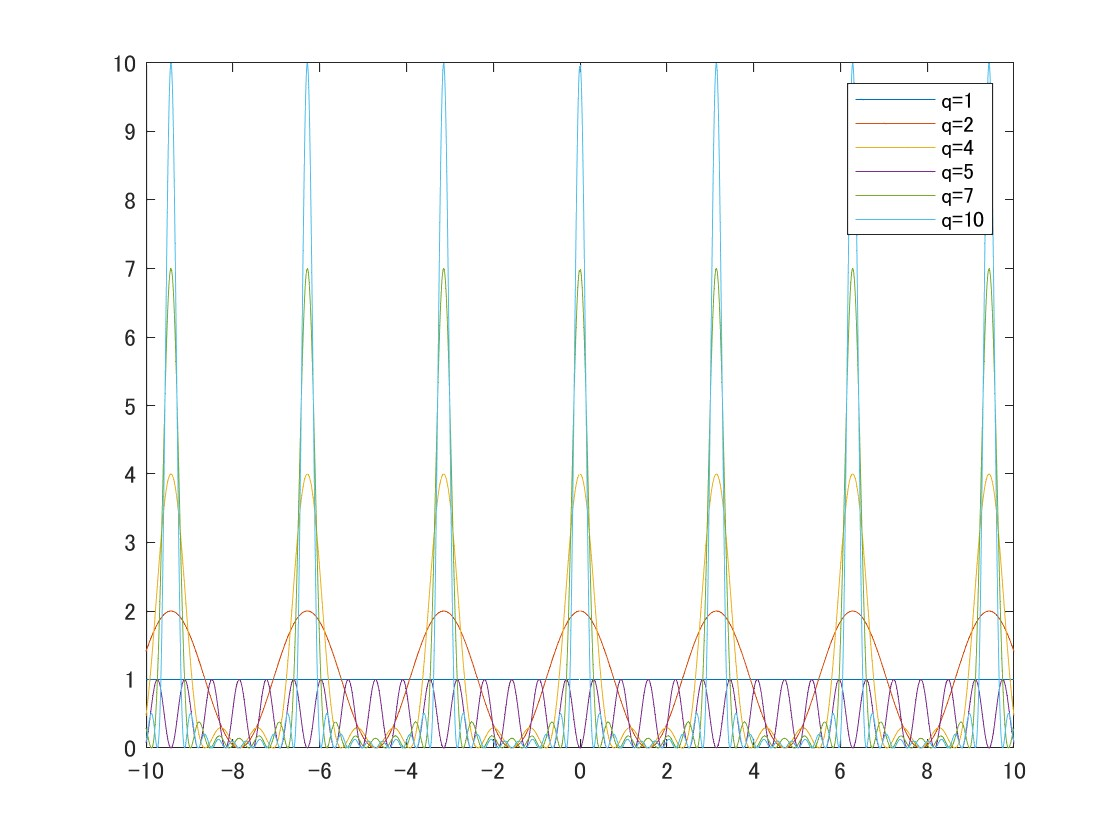
\includegraphics[width=0.8\columnwidth]{fig/neutron_diffraction.jpg}
            \caption{散乱パターン}
            \label{neutron-diffraction}
          \end{figure}
  \end{enumerate}
  \end{myexc}
  \begin{myexc}{Griffith Problem10.22 2次元散乱理論}{}
    2次元の散乱を考える.
  \begin{enumerate}
    \item 極座標ラプラシアン
    \begin{align}
      \laplacian= \frac{\partial^2}{\partial r} + \frac{1}{r}\frac{\partial}{\partial} + \frac{1}{r^2}\frac{\partial^2}{\partial \theta^2}
    \end{align}
    を用いてポテンシャル$V(r)$の下での波動関数を求めよ.ここで$u(r)=\sqrt{r}R(r)$が
    \begin{align}
      -\frac{\hbar^2}{2m}\frac{\r{d}^2 u}{\dd{r}^2} + \qty[V(r) + \frac{\hbar^2}{2m}\frac{(j^2 - 1/4)}{r^2}]u = Eu \label{eq-for-u}
    \end{align}
    を満たすことを用いてよい.$j$は整数である.
    \item $r$が十分大きいときの\refe{eq-for-u}を考えることにより,
    \begin{align}
      R(r) \sim \frac{\e^{\i kr}}{\sqrt{r}}
    \end{align}
    であることを示せ.ここで,$k\coloneqq \sqrt{2mE}/\hbar$である.
  \end{enumerate}
    \tcblower
    \begin{align}
      &\qty[-\frac{\hbar^2}{2m}\laplacian + V(r)]\psi(r,\theta) = E\psi(r,\theta)\\
      &\qty[\frac{\hbar^2}{2m}\qty(\frac{\partial^2}{\partial r^2} + \frac{1}{r}\frac{\partial}{\partial r} + \frac{1}{r^2}\frac{\partial^2}{\partial \theta^2}) + V(r)]\psi(r,\theta) = E\psi(r,\theta)
    \end{align}
    $\psi(r,\theta) = R(r)\Theta(\theta)$とし,上式を整理すると
    \begin{align}
      \frac{r^2}{R(r)}\qty(\frac{\partial^2}{\partial r^2}R(r)) - \frac{r}{R(r)}\qty(\frac{\partial}{\partial r}R(r)) + \frac{2mr^2}{\hbar^2}(V(r) - E) - \frac{1}{\Theta(\theta)} \frac{\partial^2}{\partial \theta^2}\Theta(\theta) = 0
    \end{align}
    となる.
    \begin{align}
      - \frac{1}{\Theta(\theta)} \frac{\partial^2}{\partial \theta^2}\Theta(\theta) = j^2
    \end{align}
    とすれば
    \begin{align}
      \Theta(\theta) = \e^{\i j\theta}
    \end{align}
    が得られる.さらに,
    \begin{align}
      \Theta(\theta) = \Theta(\theta + 2\pi)
    \end{align}
    だから$j$は整数であることがわかる.よって$r$に関する部分は
    \begin{align}
      \frac{r^2}{R(r)}\qty(\frac{\partial^2}{\partial r^2}R(r)) - \frac{r}{R(r)}\qty(\frac{\partial}{\partial r}R(r)) + \frac{2mr^2}{\hbar^2}(V(r) - E) = -j^2
    \end{align}
    である.整理すると
    \begin{align}
      -\frac{\hbar^2}{2m}\frac{\partial^2}{\partial r^2}R(r) - \frac{\hbar^2}{2mr}\frac{\partial}{\partial r}R(r) + (V(r) - E)R(r) + \frac{\hbar^2 j^2}{2mr^2}R(r) = 0
    \end{align}
    である.これは\refe{eq-for-u}に$u=\sqrt{r}R$を代入した式と同一である.よって波動関数は
    \begin{align}
      \psi(r,\theta) = R(r)\e^{\i j\theta}
    \end{align}
    と表されることがわかる.ただし,$j$は整数,$u=\sqrt{r}R$が
    \begin{align}
      -\frac{\hbar^2}{2m}\frac{\r{d}^2 u}{\dd{r}^2} + \qty[V(r) + \frac{\hbar^2}{2m}\frac{(j^2 - 1/4)}{r^2}]u = Eu
    \end{align}
    を満たすとする.
    
    \refe{eq-for-u}で$r\to\infty$とすれば
    \begin{align}
      -\frac{\hbar^2}{2m}\frac{\r{d}^2 u}{\dd{u}^2} = Eu
    \end{align}
    であるため,
    \begin{align}
      R(r) = \frac{u}{\sqrt{r}} = \frac{\e^{\i kr}}{\sqrt{r}}
    \end{align}
    であることがわかる.

    以上の結果は2次元の散乱問題の境界条件が
    \begin{align}
      \psi(r,\theta) \simeq \e^{\i kx} + f(\theta)\frac{\e^{\i kr}}{\sqrt{r}},\ \r{for}\ r \to \infty
    \end{align}
    であることを示唆している.また,2次元の部分波展開はHankel関数$H^{(1)}$を用いて,
    \begin{align}
      \psi(r,\theta) = \e^{\i kx} + \sum_{j} c_j H^{(1)}_j (kr) \e^{\i j\theta}
    \end{align}
    となる.
  \end{myexc}
  \begin{myexc}{Griffith example11.2}{}
    Fermiの黄金律を用いてポテンシャル$V(\bm{r})$に対する散乱断面積を求めよ.
    \tcblower
    初期状態と終状態はそれぞれ入射波と散乱波であるため
    \begin{align}
      \psi_i = \frac{1}{\sqrt{L^3}} \e^{\i \bm{k}\cdot\bm{r}}\\
      \psi_f = \frac{1}{\sqrt{L^3}} \e^{\i \bm{k}'\cdot\bm{r}}
    \end{align}
    と表される.ここで,規格化のために周期$L$の周期的境界条件を課した.また,この周期的境界条件により,
    \begin{align}
      \bm{k}' = \frac{2\pi}{L}(n_x \bm{e}_x + n_y \bm{e}_y + n_z \bm{e}_z)
    \end{align}
    が得られる.$n_x,n_y,n_z$は整数である.散乱体のポテンシャル$V(\bm{r})$を摂動として取り入れると
    \begin{align}
      \bra{f}\hat{V}\ket{i} = \int \psi_f^{*}V(\bm{r})\psi_i \dd{\bm{r}} = \frac{1}{L^3} \int \e^{\i(\bm{k} - \bm{k}')\cdot \bm{r}} V(\bm{r}) \dd{\bm{r}}
    \end{align}
    を得る.

    次に,状態密度を決定する.エネルギーが$[E,E+\dd{E}]$の状態は,厚さ$k$,立体角$\dd{\Omega}$の球殻の中に
    \begin{align}
      \frac{k^2 \dd{k} \dd{\Omega}}{(2\pi/L)^3}
    \end{align}
    個含まれている.よって,
    \begin{align}
      \rho(E) \dd{E} = \frac{k^2 \dd{k} \dd{\Omega}}{(2\pi/L)^3} = \qty(\frac{L}{2\pi})^3 k^2 \dv{k}{E} \dd{E} \dd{\Omega}
    \end{align}
    $E= \frac{\hbar^2 k^2}{2m}$なので,
    \begin{align}
      \rho(E) = \qty(\frac{L}{2\pi})^3 \frac{\sqrt{2m^3E}}{\hbar^3} \dd{\Omega}
    \end{align}
    が得られる.よって,Fermiの黄金律から,単位時間に立体角$\dd{\Omega}$に粒子が到達する確率は
    \begin{align}
      \omega_{i\to\dd{\Omega}} = \frac{2\pi}{\hbar} \frac{1}{L^6} \abs{\int \e^{\i(\bm{k} - \bm{k}')\cdot \bm{r}} V(\bm{r}) \dd{\bm{r}}}^2 \qty(\frac{L}{2\pi})^3 \frac{\sqrt{2m^3E_f}}{\hbar^3} \dd{\Omega}
    \end{align}
    である.さらに,
    \begin{align}
      \sigma \dd{\Omega} = \frac{(\text{単位時間に立体角$\dd{\Omega}$に粒子が到達する確率})}{(単位時間単位面積当たりに粒子が入射する確率)}
    \end{align}
    であり,分子は入射波の確率の流れである.これは
    \begin{align}
      J = \frac{1}{L^3}\frac{\hbar k}{m}
    \end{align}
    である.以上より,散乱断面積
    \begin{align}
      \sigma = \frac{\omega_{i\to\dd{\Omega}}}{J \dd{\Omega}} = \abs{-\frac{m}{2\pi\hbar^2}\int \e^{\i(\bm{k}' - \bm{k})\cdot\bm{r}}V(\bm{r})\dd{\bm{r}}}^2
    \end{align}
    が得られる.これは第1 Born近似で得られた式と同一である.
  \end{myexc}
\end{document}